\section{Introduction}

Gaia \citep{Prusti2016} released sparse photometry for about 157{,}000 numbered asteroids in DR3
\citep{Vallenari2023,Tanga2023}. Sparse photometry can constrain periods and spin states
\citep{Kaasalainen2004}. Several groups have derived rotation periods or spin states from DR3, notably
\citet{Durech2023}, \citet{Cellino2024} and \citet{MacLennan2026}. Many asteroids with enough transits
still have no published period.

Before such periods can be used, two things are needed. The first is a measured rate at which a period is
wrong. The second is the same rate for asteroids that are \emph{not} already in other catalogues. This
paper provides both and makes the pipeline fast enough to rerun on Gaia DR4. A pilot on 600 asteroids was
reported in \citet{Tropynin2026a}.

\section{Data and geometry}

All 20 bulk files of \texttt{sso\_observation} (23.3\,M CCD rows) were averaged per \texttt{transit\_id}.
This gives 3{,}069{,}170 transits of 156{,}789 numbered asteroids, of which 42{,}195 have at least 25
transits. Each transit carries the largest relative flux error of its CCDs, with a 0.03\,mag floor.
353 asteroids fall below 25 transits after outlier clipping and are dropped.

Heliocentric positions come from JPL osculating elements (epoch 2026 June). These were integrated back to
2014--2017 with a fourth-order Runge--Kutta scheme, a one-day step, and the Sun and the giant planets as
perturbers. Gaia's position is taken from the data, and light time is iterated. Against JPL Horizons on
19 asteroids, the reduced magnitudes agree to 0.0007\,mag.

\section{Model and search}

The reduced magnitude $G-5\log_{10}(r\Delta)$ is fitted by weighted least squares. The model has:
\begin{itemize}
\item one constant per observing season;
\item a term linear in phase angle;
\item a second-order Fourier series in the phase $2\pi(ft - s\,\lambda_{\rm PAB}/360^\circ)$.
\end{itemize}
Here $\lambda_{\rm PAB}$ is the ecliptic longitude of the phase-angle bisector seen from Gaia
\citep{Harris1984}, and $s=\pm1$ is the sense of rotation. Both senses are searched, and the better fit is
kept.

The search covers periods of 2--1000\,h on a grid with step $0.5/T$, where $T$ is the time span; the 30
deepest minima are then refined. A five times finer grid changed precision by less than a point. When the
first harmonic exceeds $1.20$ times the second, the doubled period is adopted.

The PAB correction was adopted because it is better on the tuning half. Over all solutions it raises the
fraction of correct periods from 44.2\% to 52.2\%. At probability $\ge0.8$ it increases the number of
periods from 928 to 1389 while keeping precision at 92\%. The test half shows the same effect: 45.5\% to
52.6\%. With the correction, the median difference from the sidereal periods of \citet{Durech2023} falls
by a factor of four. Without it, that difference grows with period, as an uncorrected synodic drift would.

\section{Calibration and null tests}

The truth set is LCDB V4.0 \citep{Warner2009,Warner2021} with quality $U\ge2-$. It was released in
September 2021, before Gaia DR3. A period counts as correct if it is within 3\% of the LCDB value. The
9{,}613 known asteroids were split by a hash of their number into TUNE (4{,}779) and TEST (4{,}834).

On TUNE I fitted the doubling rule and a logistic model of the probability that a period is correct. The
model uses seven features:
\begin{itemize}
\item the $\chi^2$ gain;
\item the separation from the next non-alias minimum;
\item the number of transits;
\item the amplitude;
\item the reduced $\chi^2$;
\item the period;
\item the harmonic ratio.
\end{itemize}
On TEST, the predicted probabilities match the observed fractions (Figure~\ref{fig:rel}), but the top bin is
slightly overconfident: 0.95 predicted against 0.89 observed.

The confidence threshold was not chosen on TEST. Two null tests use the real Gaia sampling but remove the
rotation:
\begin{itemize}
\item \emph{white}: residuals of the no-rotation model are permuted within seasons;
\item \emph{block}: one-day blocks of residuals are permuted, which keeps correlated systematics.
\end{itemize}
Noise periods match no catalogue, so all of them would land among the candidate new periods. The rule,
fixed in advance, is that the projected noise must stay below 5\% of that list. The probability grid
step is 0.05.

Both null tests were run on all 32{,}229 solved asteroids without an LCDB period, so the projected
noise count is simply the number that pass. At the TUNE threshold for 80\% precision (0.384), 20.0\%
(white) and 18.1\% (block) of these signal-free asteroids pass. Table~\ref{tab:null} gives the counts at
higher thresholds. Under the rule, the threshold is 0.80. There 39 (white) and 32 (block) asteroids
pass, which is 4.5\% and 3.7\% of the 861 candidate new periods. The 95\% Poisson upper limits are 51
and 43, that is 5.9\% and 5.0\%. These figures are conservative, because they treat every unknown
asteroid as having no detectable rotation.

\begin{table}
\centering
\caption{Signal-free asteroids (out of 32{,}229) that reach a given probability in the null tests.}\label{tab:null}
\begin{tabular}{ccc}
\hline
Threshold & White & Block \\
\hline
0.70 & 264 & 248 \\
0.75 & 104 & 108 \\
0.80 & 39 & 32 \\
0.85 & 12 & 8 \\
\hline
\end{tabular}
\end{table}

Tier~A is probability $\ge0.80$ and period $<100$\,h. Tier~B is probability between 0.384, the TUNE
threshold for 80\% precision, and 0.80. Tier~B is not reliable for unknown asteroids, because 18--20\% of
signal-free asteroids reach it. Periods of 100--1000\,h are flagged as slow candidates and never treated
as confident.

\section{Results}

\subsection{Periods}

6{,}238 periods reach tier~A. On TEST, 1303 of 1459 tier-A periods are correct (89.3\%): 90\%, 88\% and 83\%
at 2--10, 10--30 and 30--100\,h (Figure~\ref{fig:lcdb}).

Precision depends on the quality of the reference:
\begin{itemize}
\item 95.4\% (354/371) for $U\ge3-$;
\item 89.1\% for $U=2$ and $2+$;
\item 36\% for $U=2-$.
\end{itemize}

There are 156 disagreements:
\begin{itemize}
\item 58 differ from LCDB by exactly one cycle per day in lightcurve frequency, the daily alias of
single-site photometry;
\item 6 differ by a factor of two;
\item 92 are other periods.
\end{itemize}
For 38 of the 156 asteroids an independent TESS period exists \citep{Vavilov2025}. It agrees with this work
in 20 cases, with LCDB in 3, and with neither in 15.

The best analogue of the unknown population is the set of TEST asteroids absent from all six catalogues of
Table~\ref{tab:lit}. Tier~A is correct for 185 of 205 of them (90\%, 95\% interval 86--94\%).

\begin{table}
\centering
\caption{Agreement of tier-A periods with published catalogues (within 3\%).}\label{tab:lit}
\begin{tabular}{lccc}
\hline
Catalogue & Data & $n$ & Agree \\
\hline
\citet{Durech2023} & Gaia DR3 & 3564 & 99.6\% \\
\citet{Cellino2024} & Gaia DR3 & 2883 & 99.0\% \\
\citet{MacLennan2026} & Gaia DR3 & 2676 & 99.0\% \\
\citet{Vavilov2025} & TESS & 759 & 91.0\% \\
\citet{Erasmus2020} & ATLAS & 280 & 68.6\% \\
\citet{McNeill2023} & TESS & 863 & 55.0\% \\
\hline
\end{tabular}

\par\smallskip{\footnotesize The Gaia DR3 rows test consistency, not accuracy. For the two lower rows, agreement rises with each catalogue's own confidence. It is 81\% for
Erasmus et al.\ entries with confidence $\ge80\%$ ($n=97$). It is 77\% for McNeill et al.\ entries with
$CV_{\rm exact}\ge0.9$ ($n=419$). Factor-two relations make up $\le1.2\%$ in every row. For TEST asteroids that are also in LCDB, the two periods agree with LCDB as follows (this work vs.\ the
catalogue): 373 vs.\ 359 of 411 \citep{Vavilov2025}, 111 vs.\ 116 of 146 \citep{Erasmus2020}, and 352 vs.\
231 of 379 \citep{McNeill2023}.}
\end{table}

The $\chi^2$-curvature errors are too small. Against \citet{Durech2023}, the median $|\Delta P/P|$ is
$3.9\times10^{-5}$. Adding $5.5\times10^{-5}P$ in quadrature gives a median $|\Delta P|/\sigma\approx0.67$.
This compares two methods applied to the same data and does not include aliasing.

\subsection{Injection--recovery}

I injected synthetic double-peaked lightcurves into the real Gaia sampling of 4{,}000 asteroids without a
known period. The lightcurves had:
\begin{itemize}
\item periods of 2--100\,h, log-uniform;
\item amplitudes of 0.1--0.6\,mag, scaled by 0.5--1 per season;
\item a random spin sense, with the phase following $\lambda_{\rm PAB}$.
\end{itemize}

The real noise lies between two models. In the pessimistic model the noise is the object's own permuted
residuals; in the optimistic model it is Gaussian at the quoted errors.

Tier~A is precise under both: 96.5\% (109/113) and 99.3\% (567/571) of its periods are correct. It contains
no $P/2$ or $2P$ errors, and the spin sense is correct for 96--97\% of the correct periods.

Completeness is low, 2.7\% and 14\%, compared with 10.5\% of real unknown asteroids that reach tier~A. It
rises with amplitude and with the number of transits; no amplitude below 0.2\,mag is recovered. Tier~A is
thus a high-precision, low-completeness selection. It should not be used for population statistics
without a selection-function correction.

\subsection{Spin senses}

The sense $s$ was compared with the hemisphere of published poles, excluding poles within $20^\circ$ of the
ecliptic and ambiguous pole pairs:
\begin{itemize}
\item 3473 of 3535 agree (98.2\%) for \citet{Durech2023}, which uses the same data;
\item 3802 of 3899 agree (97.5\%) for DAMIT \citep{Durech2010};
\item 372 of 394 agree (94.4\%) for DAMIT asteroids not in \citet{Durech2023}.
\end{itemize}

The errors are nearly symmetric. Against \citet{Durech2023}, 60 prograde asteroids are called retrograde
and 44 retrograde asteroids are called prograde.

Tier~A has 3{,}677 retrograde and 2{,}561 prograde rotators (59\% retrograde). I do not interpret this
excess here, because tier~A is not an unbiased sample.

\subsection{Yarkovsky segregation in families}

The Yarkovsky drift moves prograde rotators outward and retrograde ones inward, so the two senses lie on
opposite sides of a family's V-shape \citep{Vokrouhlicky2015}. This has been shown with modelled poles
for several families \citep{Hanus2013,Hanus2018,Kryszczynska2013}.

I used AstDyS family membership and synthetic proper elements \citep{Knezevic2003,Milani2014}, with the
proper $a$ of the namesake as each family's centre. A member is consistent with the effect if it is
prograde and outside the centre, or retrograde and inside it. The right null hypothesis keeps each
family's mix of senses and its positions and breaks only the link between them. I therefore permuted the
senses within each family 20{,}000 times.

\begin{itemize}
\item \textbf{Overall.} 1{,}753 of 2{,}345 tier-A members (74.8\%) are consistent, against $52.4\pm0.9\%$
under the null hypothesis ($z=24.7$; no permutation reaches the observed value). The $2\times2$ odds ratio
is 9.1.
\item \textbf{Distance from the centre.} The fraction rises from 58\% for members near the centre to 82\% for
members whose $|a-a_c|\,D$ exceeds twice the family median, as expected for Yarkovsky drift.
\item \textbf{Choice of centre.} The result is insensitive to it: 71.3\% with the median $a$ of all members.
\item \textbf{Members without a previous pole.} The effect holds for the 912 members without a pole in
\citet{Durech2023}: 73.6\%.
\item \textbf{Individual families.} The largest families show it clearly: (221) Eos 86\% of 578, (24) Themis
81\% of 184, (15) Eunomia 79\% of 294, (158) Koronis 78\% of 184 (Figure~\ref{fig:yark}).
\end{itemize}

Random sense errors can only dilute the segregation. The observed 74.8\% therefore implies that at least
75\% of the senses are correct, a bound independent of any pole catalogue. Tier~A favours high-amplitude
rotators, so the fraction describes this subset, not complete families.

\begin{figure}
\centering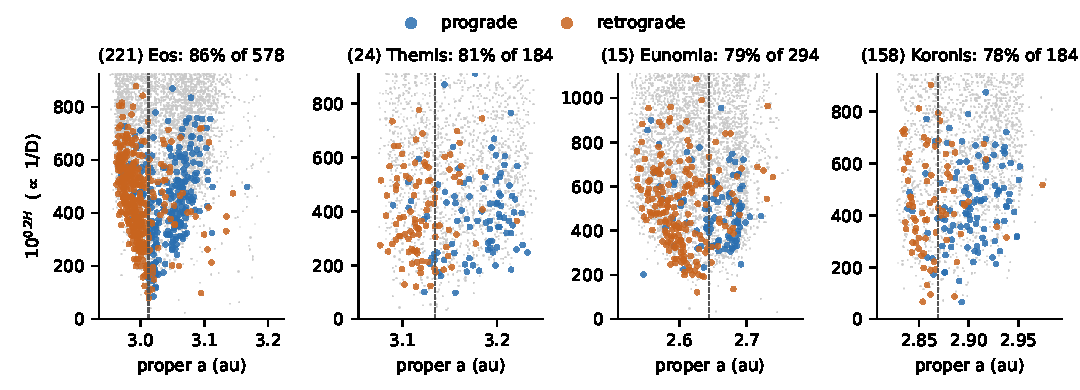
\includegraphics[width=0.95\linewidth]{fig4_yarkovsky.pdf}
\caption{Four families in proper semimajor axis against $10^{0.2H}\propto1/D$. Grey: all AstDyS members.
Blue: prograde; orange: retrograde (tier~A, this work). Dashed line: the namesake. Each title gives the
fraction of members on the side the Yarkovsky effect predicts.\label{fig:yark}}
\end{figure}

\subsection{Disputed LCDB periods}

I selected tier-A asteroids whose LCDB V4.0 period disagrees with this work and met one of two conditions:
\begin{itemize}
\item an independent survey supports this work and none supports LCDB
\citep{Vavilov2025,McNeill2023,Erasmus2020};
\item at least two other Gaia DR3 analyses support this work.
\end{itemize}
This gives 117 asteroids. Of these, 32 are exact daily aliases and 14 differ by a factor of two.

In the 2023 LCDB revision distributed by the JPL Small-Body Database, 9 of the 117 have already been
revised to the value found here. The other 108 are disputed. Of these:
\begin{itemize}
\item 39 are disputed by independent survey data and 69 by agreement of Gaia DR3 analyses only;
\item by LCDB quality, 83 have $U=2$, 9 have $U=2+$, 5 have $U=2-$, 3 have $U=3-$ and 8 have $U=3$.
\end{itemize}
The list is part of the catalogue.

\subsection{Candidate new periods}

942 tier-A asteroids have no period in LCDB or in the six catalogues. For 81 of them (8.6\%), a rotation
period exists in one of three other sources:
\begin{itemize}
\item DAMIT;
\item about 180 VizieR tables with rotation periods (5.0\,M rows), with units taken from the table metadata
and non-rotation periods excluded;
\item the Minor Planet Bulletin, volumes 50--53.
\end{itemize}
Where the values can be compared, every disagreement has an identified cause:
\begin{itemize}
\item partial-coverage PTF periods that are half of ours \citep{Chang2016};
\item K2 periods that differ by 3--6\% \citep{Sergeyev2025};
\item fast rotators below our 2\,h limit \citep{Erasmus2019};
\item two slow rotators.
\end{itemize}

The remaining 861 are candidate new periods: 667 at 2--10\,h, 131 at 10--30\,h and 63 at 30--100\,h. The
matched control gives an expected precision of about 90\%. Noise is at most 32--39 periods (3.7--4.5\%; 95\% upper limit 5.9\%). SsODNet, Behrend's Geneva page and
ZTF period papers outside VizieR were not searched. Given the 8.6\% found in the other sources, some
further candidates are likely to be already published.

The pilot list of 42 candidates \citep{Tropynin2026a} changes as follows:
\begin{itemize}
\item 35 agree with this work;
\item 4 were half the true period;
\item 3 (39932, 109412, 13686) are now ambiguous, with the extended search preferring slow solutions
outside tier~A.
\end{itemize}

\section{Limitations and plans for Gaia DR4}

\begin{itemize}
\item Periods below 2\,h are not searched.
\item The $A_1/A_2$ doubling rule is a heuristic.
\item For doubled periods the PAB coefficient should be 2. A variant that also tries 2 changed TEST precision
only from 89.3\% to 89.7\%.
\item Tumblers fall outside a single-period model.
\item Completeness is low below an amplitude of 0.3\,mag, and nothing is recovered below 0.2\,mag.
\end{itemize}

DR4 will cover about 66 months. For it, I plan to fit the sidereal period and the pole jointly on a coarse
pole grid, with a model-based test of $P$ against $2P$. Thresholds and null tests are fixed in advance, so
that results can be released within a day.

\begin{figure}
\centering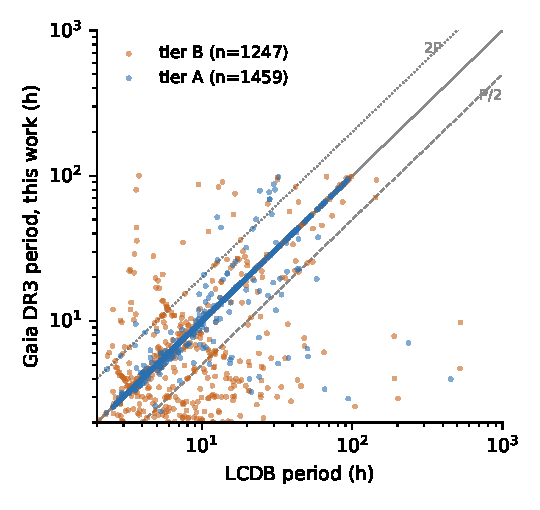
\includegraphics[width=0.95\linewidth]{fig1_lcdb.pdf}
\caption{Period from this work against the LCDB period for TEST asteroids. Blue: tier~A. Orange: tier~B
(probability 0.384--0.80). Lines mark $P$, $2P$ and $P/2$. The off-diagonal scatter includes daily aliases
in the reference periods.\label{fig:lcdb}}
\end{figure}

\begin{figure}
\centering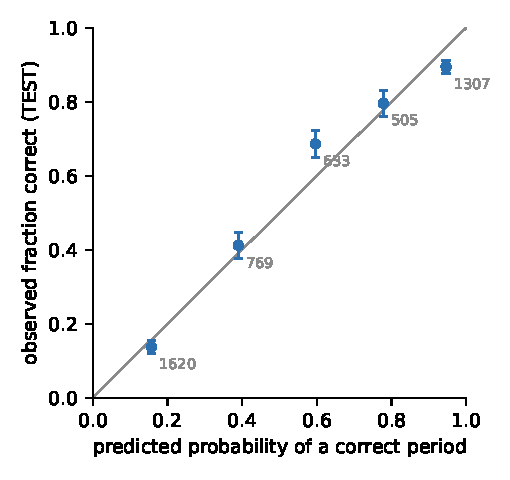
\includegraphics[width=0.95\linewidth]{fig2_reliability.pdf}
\caption{Reliability diagram on TEST for all solutions. Bars are 95\% binomial intervals; numbers give the
count per bin.\label{fig:rel}}
\end{figure}

\begin{figure}
\centering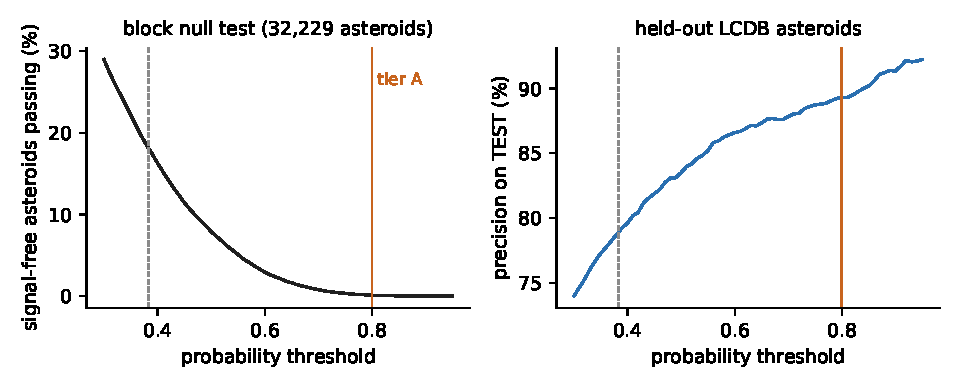
\includegraphics[width=0.95\linewidth]{fig3_threshold.pdf}
\caption{Left: fraction of signal-free asteroids (block null test) that pass, as a function of the
probability threshold. Right: precision on TEST. Dashed line: the TUNE threshold for 80\% precision. Solid
line: the tier-A threshold.\label{fig:thr}}
\end{figure}

